\documentclass[11pt]{article}

% Final version (shows author names)
\usepackage{acl}

% Standard package includes
\usepackage{times}
\usepackage{latexsym}
\usepackage[T1]{fontenc}
\usepackage[utf8]{inputenc}
\usepackage{microtype}
\usepackage{inconsolata}
\usepackage{graphicx}
\usepackage{booktabs}
\usepackage{amsmath}
\usepackage{amssymb}
\usepackage{tikz}
\usetikzlibrary{shapes.geometric, arrows.meta, positioning, fit, backgrounds, decorations.pathreplacing}

\title{CascadeMind at SemEval-2026 Task 4: A Hybrid Neuro-Symbolic Cascade \\for Narrative Similarity}

\author{Sebastien Kawada$^{\dagger,\ddagger}$ \hspace{1cm} Dylan Holyoak$^{\ddagger}$ \\
  $^{\dagger}$\,Kaons \quad $^{\ddagger}$\,Epoch Learn \\
  \texttt{sebastien@kaons.com} \quad \texttt{dylan@epochlearn.com}}

\begin{document}
\maketitle

\begin{abstract}
Across self-consistency samples from an LLM, vote agreement tracks instance difficulty: on SemEval-2026 Task 4 (Narrative Story Similarity), supermajority cases ($\geq 7/8$ votes) resolve at 85\% accuracy, split votes at 67\%, and perfect ties at 61\%, a monotone gradient that holds across the development set. We exploit this in CascadeMind, which routes eight Gemini 2.5 Flash votes by consensus, escalates split votes to additional sampling rounds, and falls through to a symbolic ensemble of theory-inspired narrative signals only on perfect ties (5\% of cases). The system reached 72.75\% on Track A test, placing \textbf{10th of 44 teams}. Ablations show the symbolic component contributes negligibly end-to-end; nearly all gains come from confidence-aware routing. The takeaway is methodological: for narrative similarity, calibrating when to spend more compute on a hard instance matters more than adding auxiliary representations to reason about it.
\end{abstract}

\section{Introduction}

Narrative similarity, the task of determining whether two stories share meaningful commonality, is a fundamental challenge in computational narratology and comparative similarity judgment \citep{piper2021narrative,tversky1977features}. SemEval-2026 Task 4 uses the comparative judgment paradigm: given an anchor story and two candidates, systems must determine which candidate is more narratively similar to the anchor \citep{hatzel-etal-2026-semeval}. Beyond surface-level text similarity, this requires understanding deeper storytelling aspects: the \emph{abstract theme} (ideas and motives), \emph{course of action} (sequence of events), and \emph{outcomes} (results and resolutions) \citep{hatzel-etal-2026-semeval}. This task design reflects how humans naturally compare stories and has applications in narrative recommendation, plagiarism detection, and literary analysis. 

While large language models (LLMs) excel at semantic understanding, previous research also demonstrates that LLMs can struggle on genuinely ambiguous cases where multiple valid interpretations exist \cite{keluskar2024llms}. To address this challenge, we take loose inspiration from decision settings in which different reasoning strategies are applied depending on task difficulty and available knowledge \cite{kahneman2011fast}. We developed a hybrid neuro-symbolic model, called \textit{CascadeMind}, by combining LLMs and rule-based symbolic reasoning \citep{garcez2023neurosymbolic}. The CascadeMind model (1) uses self-consistency-style voting \citep{wang2022self} to assess uncertainty in LLM decisions, (2) employs a supermajority threshold to identify confident vs.~uncertain predictions, and (3) defers the most uncertain decisions (perfect ties) to a symbolic ensemble module based on narrative theory for further analysis.

Our contributions are:
\begin{itemize}
    \item A cascade architecture combining neural self-consistency with rule-based symbolic reasoning
    \item A Multi-Scale Narrative Analysis Ensemble incorporating five signals from different levels of narrative abstraction that apply auxiliary reasoning to the most ambiguous cases
    \item Empirical analysis showing that cascade design provides more value than the symbolic component alone
\end{itemize}

\section{Related Work}

\paragraph{Self-Consistency Decoding}
Self-consistency is related to ensemble learning, where aggregating multiple hypotheses can improve predictions \cite{hansen2002neural}. \citet{wang2022self} introduced self-consistency as a decoding strategy that samples multiple reasoning paths and selects the most consistent answer through majority voting, showing that diverse reasoning traces yield significantly higher accuracy than single samples. Recent work also studies consistency across multiple LLM samples as a black-box uncertainty signal \citep{xiong2024uncertainty}. Self-consistency-style approaches have been extended to medical question answering \citep{maharjan2024openmedlm} and code generation \citep{huang2023enhancing}, while recent work on mirror-consistency addresses overconfidence in minority responses \citep{huang2024mirror}.

\paragraph{Narrative Representation Learning}
Computational approaches to narrative understanding draw on structural narrative theory \citep{propp1968morphology,thorndyke1977storygrammar} as well as neural embedding representations. \citet{hatzel2024story} introduced story embeddings that capture narrative similarity by training on reformulations of the same story. This work is directly relevant to our task as it comes from the task organizers. The CoRRPUS framework \citep{dong2023corrpus} showed that structured code-based representations can improve story understanding in a neurosymbolic setting.

\paragraph{Ensemble Methods and Selective Prediction}
\citet{dietterich2000ensemble} shows that ensembles can classify data points by weighted voting of predictions. Selective prediction allows models to abstain when uncertain, trading coverage for accuracy \citep{geifman2017selective}. Our cascade borrows from selective prediction by using uncertainty to choose a downstream decision path, while still returning a prediction for every case.

\paragraph{Narrative Theory}
Our symbolic component draws on classical narrative theory. Propp's morphology of the folktale \citep{propp1968morphology} identified recurring structural elements across stories. Freytag's pyramid models narrative tension through exposition, rising action, climax, falling action, and resolution \citep{freytag1894technik}. Todorov's narrative grammar \citep{todorov1969grammaire} analyzes structured transformations in narrative. We operationalize these theories as computable similarity signals.


\section{System Architecture}
CascadeMind uses a direct comparative prompt aligned with the task definition. The prompt asks which candidate story is more similar to the anchor, focuses the decision on abstract theme, course of action, and outcomes, then provides the anchor, Story A, and Story B. The model is instructed to return JSON with a \texttt{decision} field set to either \texttt{A} or \texttt{B}; no chain-of-thought rationale is requested or used.

Our system implements a four-stage routing pipeline that combines neural voting with symbolic rule-based reasoning for the most uncertain cases. Figure~\ref{fig:architecture} illustrates the overall architecture.

\begin{figure}[!htb]
\centering
\small
\setlength{\tabcolsep}{3pt}
\begin{tabular}{c}
\textbf{Stage 1: Self-Consistency Voting} \\[4pt]
$\mathcal{V} = \{v_1, \ldots, v_8\} \quad v_i \sim \text{LLM}(x_{\text{anchor}}, x_A, x_B)$ \\[6pt]
\hline \\[-6pt]
\textbf{Stage 2: Confidence Check} \\[6pt]
{\scriptsize$\hat{y} = \left\{
\begin{array}{@{}ll@{}}
\operatorname*{argmax}_{X} |\{v_i = X\}| & \text{if } \max_X |\{v_i = X\}| \geq 7 \\[2pt]
\textsc{Escalate} & \text{otherwise}
\end{array}
\right.$} \\[12pt]
\hline \\[-6pt]
\textbf{Stage 3: Escalation (if needed)} \\[4pt]
$\mathcal{V}' = \mathcal{V} \cup \{v_9, \ldots, v_{32}\} \quad \hat{y} = \text{majority}(\mathcal{V}')$ \\[6pt]
\hline \\[-6pt]
\textbf{Stage 4: Symbolic Tiebreaker (if $|\mathcal{V}'_A| = |\mathcal{V}'_B|$)} \\[4pt]
$\hat{y} = \arg\max_X \sum_{i=1}^{5} w_i \cdot \text{sim}_i(x_{\text{anchor}}, x_X)$
\end{tabular}

\vspace{6pt}
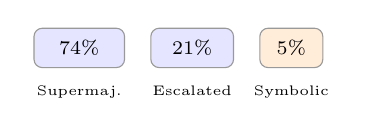
\begin{tikzpicture}[
    node distance=0.4cm,
    box/.style={rectangle, rounded corners=3pt, minimum height=0.5cm, draw=black!40, fill=#1, font=\scriptsize, text centered},
    arrow/.style={-{Stealth[scale=0.6]}, draw=black!40}
]
\node (s1) [box=blue!10, minimum width=1.15cm] {74\%};
\node (s2) [box=blue!10, minimum width=1.05cm, right=0.32cm of s1] {21\%};
\node (s3) [box=orange!15, minimum width=0.8cm, right=0.32cm of s2] {5\%};
\node[font=\tiny, below=0.1cm of s1] {Supermaj.};
\node[font=\tiny, below=0.1cm of s2] {Escalated};
\node[font=\tiny, below=0.1cm of s3] {Symbolic};
\end{tikzpicture}
\caption{Cascade decision process. Most cases (74\%) resolve via supermajority; 21\% require escalation; 5\% invoke the symbolic ensemble.}
\label{fig:architecture}
\end{figure}

\subsection{Neural Self-Consistency Voting}

We use Gemini 2.5 Flash as our base LLM \citep{google-gemini-2-5-flash-2025}, leveraging its native \texttt{candidateCount} parameter to return eight candidate responses per API call through the Gemini API \citep{google-generative-ai-api-2025}. Each response provides a binary decision (A or B) for which story is more similar to the anchor.

\paragraph{Decision Logic}
Let $V = \{v_1, \ldots, v_8\}$ be the set of votes where $v_i \in \{A, B\}$. We define the vote count $c_X = |\{v_i : v_i = X\}|$ for $X \in \{A, B\}$.

\textbf{Supermajority:} If $\max(c_A, c_B) \geq 7$, we return the majority decision immediately. This threshold (87.5\%) indicates high model confidence.

\textbf{Escalation:} If votes are split (5-3, 6-2, or 4-4), we request three additional independent API calls, each using the model's \texttt{candidateCount=8} setting. Votes from all calls are compiled, totaling 32 votes. The majority across all votes determines the decision, unless a perfect tie (16-16 votes) occurs.

\subsection{Multi-Scale Narrative Analysis Ensemble}

When neural voting produces a perfect tie after escalation, we invoke a symbolic ensemble component combining five theory-inspired narrative signals and text-similarity signals at different levels of abstraction (Figure~\ref{fig:ensemble}). Let $s_i^A$ and $s_i^B$ denote the similarity scores between the anchor and stories A and B for signal $i$.

\begin{figure}[!htb]
\centering
\small
\fbox{\parbox{0.94\columnwidth}{
\vspace{2pt}
\textbf{Ensemble Decision:}
\vspace{-6pt}
\[
\hat{y}=\operatorname*{argmax}_{X\in\{A,B\}}\sum_{i=1}^{5}w_i\,s_i(x_{\mathrm{anc}},x_X)
\]
\vspace{-8pt}
\vspace{4pt}
\hrule
\vspace{4pt}
\begin{tabular}{@{}r@{\;}l@{\quad}l@{}}
$s_1$ & $= \cos(\mathbf{t}_{\text{anc}}, \mathbf{t}_X)$ & {\footnotesize TF-IDF vectors \hfill $w_1{=}0.49$} \\[3pt]
$s_2$ & $= \frac{1}{5}\sum\limits_{p=1}^{5} \cos(\mathbf{e}_{p}^{\text{anc}}, \mathbf{e}_{p}^{X})$ & {\footnotesize Story grammar \hfill $w_2{=}0.40$} \\[5pt]
$s_3$ & $= \cos(\mathbf{e}_{\text{anc}}, \mathbf{e}_X)$ & {\footnotesize Semantic emb. \hfill $w_3{=}0.08$} \\[3pt]
$s_4$ & $= \text{corr}(\tau_{\text{anc}}, \tau_X)$ & {\footnotesize Tension curve \hfill $w_4{=}0.02$} \\[3pt]
$s_5$ & $= \frac{2 \cdot \text{LCS}(E_{\text{anc}}, E_X)}{|E_{\text{anc}}| + |E_X|}$ & {\footnotesize Event chain \hfill $w_5{=}0.01$}
\end{tabular}
\vspace{2pt}
}}
\vspace{4pt}

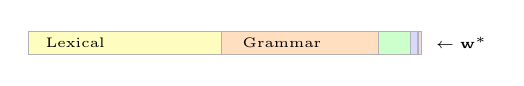
\begin{tikzpicture}
\draw[fill=yellow!25, draw=black!30] (0,0) rectangle (2.45,0.3);
\draw[fill=orange!25, draw=black!30] (2.45,0) rectangle (4.45,0.3);
\draw[fill=green!20, draw=black!30] (4.45,0) rectangle (4.85,0.3);
\draw[fill=blue!15, draw=black!30] (4.85,0) rectangle (4.95,0.3);
\draw[fill=purple!15, draw=black!30] (4.95,0) rectangle (5,0.3);
\node[font=\tiny, anchor=west] at (0.1,0.15) {Lexical};
\node[font=\tiny, anchor=west] at (2.6,0.15) {Grammar};
\node[font=\tiny] at (5.5,0.15) {$\leftarrow \mathbf{w}^*$};
\end{tikzpicture}

\caption{Multi-Scale Narrative Ensemble with five weighted similarity signals ($\mathbf{w}^*$ optimized via differential evolution).}
\label{fig:ensemble}
\end{figure}

\paragraph{Signal 1: Lexical Similarity (TF-IDF)}
We compute TF-IDF \cite{salton1988term} vectors, which represent narratives as numerical feature vectors based on word usage and importance. For each problem, we compute TF-IDF vectors for anchor narrative and the two option narratives, and then measure cosine similarity between the anchor and option narratives:
\begin{equation}
s_{\text{lex}}^X = \cos(\text{tfidf}(\text{anchor}), \text{tfidf}(X))
\end{equation}
This TF-IDF-based lexical similarity captures surface-level overlap in word usage, reflecting shared situations, characters, or domain-specific terminology.

\paragraph{Signal 2: Story Grammar Similarity}
As a heuristic inspired by story-grammar and narrative-phase models \citep{propp1968morphology,freytag1894technik,thorndyke1977storygrammar}, we segment each story into five narrative phases based on position: setting (first 20\%), conflict (20-40\%), rising action (40-60\%), climax (60-80\%), and resolution (80-100\%). We compute sentence-transformer embeddings for each aligned phase, then compute story-grammar similarity via cosine similarity:
\begin{equation}
s_{\text{grammar}}^X = \frac{1}{5}\sum_{p \in P} \cos(\text{enc}(a_p), \text{enc}(x_p))
\end{equation}
where $P$ = \{setting, conflict, rising, climax, resolution\}.

\paragraph{Signal 3: Semantic Similarity}
Using the all-MiniLM-L6-v2 sentence transformer that encodes narratives into dense vector embeddings \citep{reimers2019sentence,reimers2020allminilm}, we compute pairwise cosine similarity between the resulting embeddings:
\begin{equation}
s_{\text{sem}}^X = \cos(\text{enc}(\text{anchor}), \text{enc}(X))
\end{equation}
This measure captures overall semantic similarity in the narrative content.

\paragraph{Signal 4: Narrative Tension Curve}
Inspired by Freytag's pyramid \cite{freytag1894technik} and computational work on sentiment-derived story arcs \citep{reagan2016emotionalarcs}, we use a heuristic positional tension proxy. For each sentence, we compute a tension score as the sum of sentiment intensity (absolute polarity) and subjectivity using TextBlob \cite{loria2018textblob}. We interpolate sentence tension to a fixed-length curve of 10 points via linear interpolation, and then compute correlation between anchor and option narratives:
\begin{equation}
s_{\text{tension}}^X = \text{corr}(T_{\text{anchor}}, T_X)
\end{equation}
This procedure captures similarity in emotional dynamics and pacing.

\paragraph{Signal 5: Event Chain Similarity}
We extract action verbs using spaCy's part-of-speech tagger \citep{spacy-2025}, filtering to verbs matching a list of 47 narrative action words inspired by event-chain modeling and Propp's character functions \citep{chambers2008narrativechains,propp1968morphology} (e.g., \emph{discover}, \emph{fight}, \emph{escape}, \emph{transform}). These form event sequences $E_{\text{anc}}$ and $E_X$ (ordered verb lemmas). We compute the longest common subsequence (LCS):
\begin{equation}
s_{\text{event}}^X = \frac{2 \cdot \text{LCS}(E_{\text{anc}}, E_X)}{|E_{\text{anc}}| + |E_X|}
\end{equation}
This procedure approximates plot-structure similarity using ordered action-verb overlap.


\paragraph{Weighted Ensemble}
The final pairwise similarity is determined using a weighted sum of the above five similarity scores:
\begin{equation}
\text{score}^X = \sum_{i=1}^{5} w_i \cdot s_i^X
\end{equation}
The model returns option A if $\text{score}^A > \text{score}^B$ and option B if $\text{score}^B > \text{score}^A$; exact score ties use the implementation's deterministic option-B fallback.

We estimated ensemble weights $w_i$ using differential evolution optimization algorithm \citep{storn1997differential} on the organizer-provided synthetic SemEval-2026 Task 4 data comprising 1,900 narrative triplets \citep{hatzel-etal-2026-semeval,narrative-similarity-data-2026}. This split is LLM-generated and is used only for calibrating symbolic weights; development and test reporting in this paper uses the task's human-labeled splits.

The optimization objective minimizes classification error:
\begin{equation}
\mathbf{w}^* = \arg\min_{\mathbf{w}} \sum_{j=1}^{N} \mathbf{1}\Big[\text{sign}\big(\textstyle\sum_{i} w_i \Delta s_i^j\big) \neq y_j\Big]
\end{equation}
where $\Delta s_i^j = s_i^A - s_i^B$ and $y_j \in \{-1, +1\}$ is the ground truth label. We use differential evolution due to its effectiveness on non-convex, non-differentiable objectives. 

The optimized weights are shown in Figure~\ref{fig:ensemble}. The dominance of lexical (49\%) and story grammar (40\%) signals suggests that narrative similarity in the training data operates primarily at surface and structural levels. The ensemble achieves 99.5\% accuracy on a held-out synthetic validation split (n=200).

\section{Experiments}

\subsection{Dataset}

The SemEval-2026 Task 4 dataset and evaluation protocol are described by the task organizers \citep{hatzel-etal-2026-semeval,narrative-similarity-dataset-2026,narrative-similarity-data-2026}. All story summaries and labels used in this work are in English. The task uses Wikipedia plot synopses from the English portion of Tell-Me-Again, filtered primarily to short summaries of four to eight sentences \citep{hatzel-etal-2026-semeval}. For development analysis, we use the Track A development split of 200 story triplets. The official Track A test split contains 400 triplets. Each triplet contains an anchor story and two candidate stories, with labels indicating which candidate is more narratively similar to the anchor. The synthetic training set comprises 1,900 LLM-generated triplets and is used only for symbolic-weight calibration.

\subsection{Implementation Details}

We use Gemini 2.5 Flash via the Google AI API \citep{google-generative-ai-api-2025} with \texttt{candidateCount=8} for multi-candidate voting. Temperature is set to 1.0 to encourage response diversity. All other parameters remained set at default. The symbolic ensemble module uses scikit-learn for TF-IDF vectorization \citep{pedregosa2011scikit}, sentence-transformers (all-MiniLM-L6-v2) for embeddings \citep{reimers2019sentence,reimers2020allminilm}, and TextBlob for sentiment analysis \citep{loria2018textblob}.

\subsection{Results}

\subsubsection{Official Shared-Task Result}
Our official final shared-task result is reported in Table~\ref{tab:official_results}, as provided by the SemEval-2026 Task 4 organizers \citep{hatzel-etal-2026-semeval,narrative-similarity-results-2026}. The task received 71 final submissions from 46 teams across both tracks; Track A lists 44 ranked teams, with CascadeMind placing \textbf{10th of 44}.

\begin{table}[t]
\centering
\small
\begin{tabular}{lccc}
\toprule
\textbf{System} & \textbf{Track} & \textbf{Test Accuracy} & \textbf{Rank} \\
\midrule
CascadeMind & A & 72.75\% & \textbf{10th/44} \\
\bottomrule
\end{tabular}
\caption{Official shared-task result for our final submission, as listed in the SemEval-2026 Task 4 overview paper and official results page \citep{hatzel-etal-2026-semeval,narrative-similarity-results-2026}. Rank is among the 44 Track A teams.}
\label{tab:official_results}
\end{table}

\subsubsection{Post-Hoc Test-Set Analysis}
After release of Track A test labels \citep{narrative-similarity-dataset-2026}, we performed a post-hoc diagnostic evaluation on an archived local Track A prediction file. This analysis is intended for error characterization and does not change the official shared-task standing in Table~\ref{tab:official_results}. The archived local file obtains 73.0\% accuracy (292/400), while the official submitted file corresponds to 72.75\% (291/400), i.e., a one-prediction difference.

\begin{table}[t]
\centering
\small
\begin{tabular}{lrr}
\toprule
\textbf{Gold Label} & \textbf{Pred A} & \textbf{Pred B} \\
\midrule
A closer ($n{=}208$) & 143 & 65 \\
B closer ($n{=}192$) & 43 & 149 \\
\bottomrule
\end{tabular}
\caption{Post-hoc confusion matrix on released Track A test labels (n=400).}
\label{tab:test_confusion}
\end{table}

Class-wise behavior is asymmetric. For the \emph{A-closer} class, precision/recall/F1 are 76.9\%/68.8\%/72.6\%; for \emph{B-closer}, they are 69.6\%/77.6\%/73.4\%. Macro-F1 is 73.0\% and balanced accuracy is 73.2\%. The model predicts B more often than A (53.5\% vs. 46.5\%), while the released label distribution is slightly A-leaning (52.0\% A, 48.0\% B), indicating a mild tendency to over-select B in uncertain comparisons.

\subsubsection{Development-Set Analysis}
Table~\ref{tab:dev_results} presents development diagnostics with different denominators: baselines are computed on the full development split (n=200), while cascade routing diagnostics are computed on a separate subset (n=100). CascadeMind reaches 81.0\% on the cascade subset. Because these denominators differ, cross-block percentage-point differences are descriptive only. With 74\% resolved at supermajority and 26\% escalated to three additional calls, expected API usage is 1.78 calls per case.

Prompt variants explored during development are treated as exploratory rather than official evidence. The results reported here rely on direct A/B decisions without exposing chain-of-thought rationales.

\begin{table}[t]
\centering
\footnotesize
\begin{tabular}{@{}p{0.50\linewidth}cc@{}}
\toprule
\textbf{System} & \textbf{Accuracy} & \textbf{Calls/Case} \\
\midrule
Single Vote & 68.0\% & 1.0 \\
Self-Consistency (k=8) & 76.5\% & 1.0 \\
Majority (k=3 calls) & 78.0\% & 3.0 \\
\midrule
CascadeMind & 81.0\% & 1.78 avg \\
\quad + Symbolic Tiebreaker & 81.0\% & 1.78 avg \\
\bottomrule
\end{tabular}
\caption{Development-set system comparison (n=200 for baselines, n=100 for cascade experiments).}
\label{tab:dev_results}
\end{table}



\subsubsection{Performance by Decision Pathway}
On the development set, we examined how performance varies by decision pathway. As shown in Table~\ref{tab:ablation}, the supermajority pathway achieves 85\% accuracy, supporting the use of vote consensus as a confidence signal. Escalated cases resolved by majority achieve 67\% accuracy, while a separate perfect-tie diagnostic set attains 61\% accuracy after symbolic processing. These pathway diagnostics are consistent with the hypothesis that vote-distribution uncertainty correlates with task difficulty and with prior work using multi-sample consistency as an uncertainty signal \citep{xiong2024uncertainty}.

\begin{table}[t]
\centering
\footnotesize
\begin{tabular}{@{}p{0.47\linewidth}cc@{}}
\toprule
\textbf{Pathway} & \textbf{Cases} & \textbf{Accuracy} \\
\midrule
Supermajority ($\geq$7/8) & 74/100 & 85\% \\
Escalated (majority) & 21/100 & 67\% \\
Escalated (symbolic tie) & 5/100 & 61\% (11/18) \\
\midrule
\textit{Total} & \textit{100/100} & \textit{81\%} \\
\bottomrule
\end{tabular}
\caption{Performance breakdown by decision pathway. Routing shares are measured on the cascade diagnostic subset (n=100); symbolic-tie accuracy is measured on a separate perfect-tie diagnostic set (n=18).}
\label{tab:ablation}
\end{table}



\subsubsection{Symbolic Tiebreaker Analysis}

On the separate perfect-tie diagnostic set (n=18), the symbolic tiebreaker achieves 61.1\% accuracy (11/18; Table~\ref{tab:ablation}). Manual inspection suggests recurring errors involving misleading lexical overlap, non-standard narrative structures that violate positional assumptions, and edge cases that require world knowledge beyond surface signals. When applied to all cases regardless of neural confidence in the original cascade diagnostic subset, accuracy drops to 53\%, suggesting that the symbolic signals are best treated as a high-uncertainty fallback rather than a stand-alone classifier.

\begin{table}[t]
\centering
\footnotesize
\begin{tabular}{@{}lcccc@{}}
\toprule
\textbf{Split} & \textbf{n} & \textbf{Acc.} & \textbf{F1} & \textbf{A/B} \\
\midrule
Dev & 200 & 57.0\% & 57.0 & 99/101 \\
Test & 400 & 60.5\% & 60.4 & 208/192 \\
\bottomrule
\end{tabular}
\caption{Post-hoc symbolic-only support check using the fixed paper weights and no LLM calls.}
\label{tab:symbolic_only}
\end{table}

The full-split symbolic-only runs in Table~\ref{tab:symbolic_only} provide additional support for the symbolic module as an above-chance fallback: 57.0\% on Track A development (114/200) and 60.5\% on released Track A test labels (242/400). Prediction rates remain balanced on both splits, while the absolute accuracy remains below the neural cascade, preserving the main conclusion that voting and escalation drive the system's strongest performance.


\section{Discussion}

\paragraph{Test-Time Behavior}
Table~\ref{tab:official_results} summarizes official shared-task standing, while Table~\ref{tab:test_confusion} shows class-level behavior for the archived local file used in post-hoc analysis. The dominant test-time error is predicting B when A is correct (65 cases), which is consistent with lower recall on the A-closer class than on the B-closer class.

\paragraph{Value of Cascade Design}
On the development set, the cascade architecture's primary gains arise from the voting and escalation mechanism rather than the symbolic tiebreaker. The supermajority threshold effectively identifies confident predictions (85\% accuracy on 74\% of cases), while escalation provides additional signal for borderline cases. The key insight is that LLM vote distribution serves as a useful uncertainty indicator in this diagnostic setting: higher consensus correlates with higher accuracy, consistent with broader evidence that multi-sample consistency can support black-box LLM uncertainty estimation \citep{xiong2024uncertainty}.

\paragraph{Domain Mismatch}
The symbolic ensemble achieves 99.5\% accuracy on a held-out synthetic validation split but only 61.1\% on the perfect-tie diagnostic set, and overall system performance drops from 81.0\% on the cascade diagnostic subset to 72.75\% on official test. This gap is consistent with distribution mismatch, overfitting to synthetic calibration data, or greater difficulty in the final shared-task setting.

\paragraph{Signal Complementarity}
In this symbolic ensemble trained on synthetic data, optimized weights favor lexical (TF-IDF, 49\%) and structural (Story Grammar, 40\%) signals over semantic embeddings (8\%). However, the non-zero semantic weight indicates a minor but distinct contribution to ensemble predictions.

\paragraph{Measure Limitations}
The minimal weight for event chain similarity (1\%) likely reflects sparsity caused by exact verb matching against a finite 47-word list. This result highlights a need for richer event representations via fuzzy matching, narrative event chains \citep{chambers2008narrativechains}, or semantic role labeling.

\section{Conclusion}

We presented a hybrid neuro-symbolic cascade model for narrative story similarity that combines neural self-consistency-style voting with a Multi-Scale Narrative Analysis Ensemble. In official shared-task evaluation, CascadeMind reaches 72.75\% Track A test accuracy (Table~\ref{tab:official_results}) \citep{hatzel-etal-2026-semeval,narrative-similarity-results-2026}. On development diagnostics (cascade subset n=100), the same architecture reaches 81.0\% accuracy through a cascade that routes confident predictions immediately while escalating uncertain cases.

The main contributions are: (1) a cascade architecture showing that LLM vote distribution can serve as a useful uncertainty indicator, with development-set supermajority predictions achieving 85\% accuracy; (2) a Multi-Scale Narrative Analysis Ensemble that combines theory-inspired narrative signals and text-similarity signals; and (3) an analysis of development-to-test behavior showing a measurable generalization gap in final shared-task conditions.

\section*{Limitations}

The system depends on a commercial API (Gemini 2.5 Flash) and stochastic decoding. While the routing policy and thresholds are fixed, exact vote distributions can vary across runs and model revisions, which limits strict reproducibility without pinned model snapshots \citep{pineau2021reproducibility,chen2024chatgptbehavior}. Public code is released at \href{https://github.com/epoch-learn/CascadeMind}{epoch-learn/CascadeMind}, but shared-task data and generated submission artifacts should be retrieved from the task source unless redistribution permission is confirmed.

The development-to-test gap is substantial. Accuracy is 81.0\% on the cascade diagnostic subset (n=100) versus 72.75\% (291/400) in official shared-task evaluation. A post-hoc run on an archived local file scored 73.0\% (292/400), reflecting a one-prediction difference from the submitted file.

The symbolic tiebreaker has narrow end-to-end impact because only 5\% of the cascade diagnostic subset reaches the final tie state. Most gains come from neural voting and escalation rather than symbolic resolution, so improvements to confidence calibration and escalation strategy are likely to matter more than additional symbolic feature engineering.

Post-hoc test analysis shows asymmetric class behavior: recall is lower for A-closer cases (68.8\%) than for B-closer cases (77.6\%), and the model predicts B slightly more often than the label distribution warrants. Reducing this decision bias is a direct target for future versions.

\section*{Ethics Statement}

This work uses public story summaries and organizer-provided labels; we did not recruit, interact with, or collect data from human subjects \citep{hatzel-etal-2026-semeval,narrative-similarity-dataset-2026}. The LLM component may inherit biases and other risks present in its training data and commercial LLM deployment settings \citep{weidinger2022taxonomy}.

\section*{Acknowledgements}

We thank the SemEval-2026 Task 4 organizers \citep{hatzel-etal-2026-semeval,narrative-similarity-dataset-2026} for creating this challenging benchmark for narrative similarity and for their efforts in organizing the shared task.

\bibliography{references}

\end{document}
